%!TEX root = ../report.tex

% 
% Architecture
% 

\section{Architecture}
\label{sec:arch}

The problem addressed in this thesis is to design and implement an interactive programming environment for generative design that covers the needs of both beginners and advanced users. Our approach suggests two interactive tools: (1) \textit{sketch-correlation tool}, which correlates sketches with code, as a result it allows programmers to effortlessly read the code, and (2) \textit{immediate feedback tool}, which executes the program upon changes, thereby creating an interactive environment to users quickly test their ideas and, eventually, improve program comprehension. The next section shows how these features will work.

\subsection{Experimental results}

An initial prototype was devised to show how code and images can be correlated, as shown in Figure~\ref{fig:img-code}. In this prototype, the meaning of the function and its parameters are transparent, because users can move the mouse over an identifier to figure out its meaning. For example in the Figure~\ref{fig:img-code1}, there are two arrows pointing to the identifier \texttt{r}, when we look at the image is easy to see that it represents the radius of the sphere, while the other arrow refers to the location where it is used, i.e. in the \texttt{sphere} function. Especially in this example, the sketch illustrates exactly the function output. The function uses a primitive of Rosetta~\cite{lopes2011portable} (the \texttt{sphere} function) which creates a sphere, given a 3D point and a radius, in the selected \textit{backend}.

\begin{figure}
 \vspace{-10pt}
        \centering
        \begin{subfigure}{0.5\textwidth}
                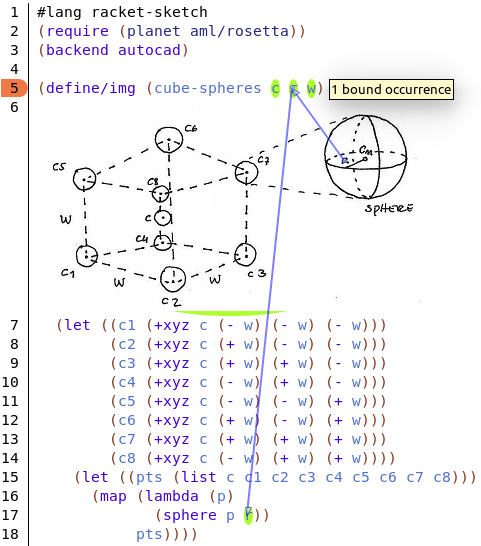
\includegraphics[width=\textwidth]{img/img-code}
                \caption{Searching for ``r'' meaning.}
                \label{fig:img-code1}
        \end{subfigure}%
        ~ %add desired spacing between images, e. g. ~, \quad, \qquad, \hfill etc.
          %(or a blank line to force the subfigure onto a new line)
        \begin{subfigure}{0.5\textwidth}
                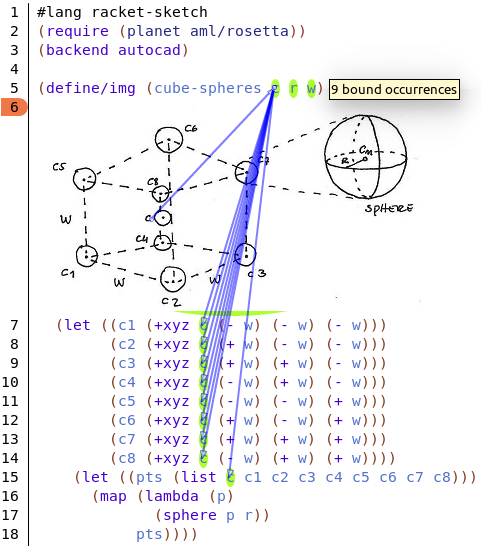
\includegraphics[width=\textwidth]{img/img-code-2}
                \caption{Searching for ``c'' meaning.}
                %\label{}
        \end{subfigure}
        \vspace{-5pt}
        \caption{Contextualizing the code with image.}
        \label{fig:img-code}
         \vspace{-10pt}
\end{figure}

\begin{figure}[htb]
 \vspace{-5pt}
    \centering
        \begin{subfigure}{0.65\textwidth}
                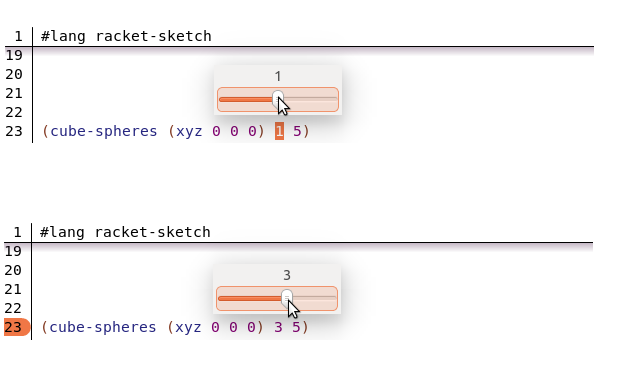
\includegraphics[width=\textwidth]{img/cube}
                \caption{Changing the ``r'' parameter.}
                \label{fig:slider1}
        \end{subfigure}%
        ~ %add desired spacing between images, e. g. ~, \quad, \qquad, \hfill etc.
          %(or a blank line to force the subfigure onto a new line)
        \begin{subfigure}{0.35\textwidth}
                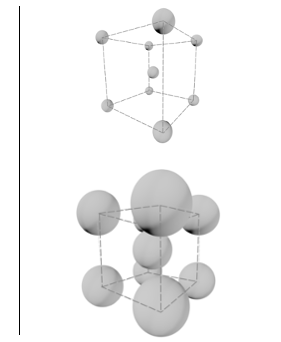
\includegraphics[width=\textwidth]{img/img-cube}
                \caption{The generated models, rendered by AutoCAD.}
                \label{fig:cube}
        \end{subfigure}
        \vspace{-5pt}
        \caption{Interacting with the \texttt{cube-spheres} function.}
        \label{fig:slider}
 \vspace{-10pt}
\end{figure}

Using the immediate feedback tool, programmers can test their ideas by quickly experiment them. The Figure~\ref{fig:slider}, shows a prototype which supports this process. In this prototype, the function defined in Figure~\ref{fig:img-code}, i.e. \texttt{cube-spheres}, is being interactively tested. Each change in the slider causes an execution of the program with the new slider value, particularly in this example, it will generate a new geometric model (see Figure~\ref{fig:cube}). As a result, users can confirm that the parameter \texttt{r} is, indeed, the radius of the sphere and it also eliminates the cycle edit-compile-run, allowing fast visualization of changes.  

These features will be built on top of DrRacket~\cite{findler2002drscheme}. In the following sections, we will present relevant properties of DrRacket that justify its choice as the basis of this thesis, as well as the proposed architecture to extend the DrRacket environment.

\subsection{DrRacket Properties}

Like DrRacket, our solution initially will target students, but, eventually, it would be used by anyone who wants to document the code with images or develops a program interactively. Therefore, to implement our solution we choose DrRacket, because it is built in the same principle we search for and has some key qualities:

\begin{itemize}
	\item \textbf{Pedagogic.} DrRacket is a popular environment used in introductory courses for programming languages. The environment is designed to guide the student by catching typical mistakes and explaining them in terms that students understand. It is also useful for professional programmers, due to its sophisticated programming tools, such as the static debugger, and its advanced language features, such as \textit{units} and \textit{mixins}.

	\item \textbf{Sophisticated editor.} DrRacket fully integrates a graphics-enriched editor which supports, in addition to plain text, elements such as images and boxes (with comments, Racket code or XML code). DrRacket also displays these elements appropriately in its read-eval-print loop.

	\item \textbf{Extensible.} The main tools of the DrRacket environment are implemented using the same \ac{api} that is available for extension. For example, the debugger, the syntax checker and the stepper, despite providing different functionalities, are implemented on top of the same \ac{api}.
\end{itemize}

Moreover, DrRacket helps programmers to understand the syntactic and lexical structure of their programs. DrRacket provides a syntax checker that annotates a syntactically correct program in five categories: the primitives, keywords, bound variables, free variables, and constants. When the programmer moves the mouse over an annotated identifier, the syntax checker displays arrows that point from bound identifiers to their binding occurrence, and vice-versa (see Figure~\ref{fig:img-code}). However, the syntax checker ignores the category of comments, including its visual elements such as the images, as a result these elements are uncorrelated with the program's structures and behavior.

In the next section, we propose an architecture which aims to address the above issue as well as proposes a solution for the immediate feedback tool.

\subsection{Proposed Architecture}

Figure~\ref{fig:solution} presents a publish-subscribe view of the proposed features. There are two different interactions in this architecture, the first presented by a publish-subscribe and the second by a client-server.

\begin{enumerate}
	\item The main functionality of the proposed environment is made through a publish-subscribe interaction. The \texttt{DrRacket UI event manager} acts as an event bus for user-interface events (such as button clicks). From this event bus we subscribe only the \ac{ui} events which are relevant to our system, defining which components will handle them. It is done at load time when the event manager reads the \textit{plugin} configuration file (\texttt{info} file). When users are working on the editor, an \ac{ui} event is generated and dispatched via implicit invocation to the action handler objects that subscribe to that event.

	\item The client-server interaction is only needed to support the correlation between images and code. We assume that the images, inserted in the editor, will be associate to a single function and will contain the same identifiers defined by its associated function parameters (as shown the handmade sketch in Figure~\ref{fig:img-code}). Then, the manuscript symbols present in the image (e.g. the parameters ``c'',``r'', and ``w''), will be parsed using an \ac{ocr} engine. This engine usually gets an image and returns a text file containing a symbol table with the parsed symbols and its respective coordinates. We expect the \ac{ocr} engine to act as an external service that identifies those symbols, thereby in our architecture the \texttt{symbol identifier} component calls this service to handle the recognition of symbols in the image.
\end{enumerate}

\begin{figure}[htb]
 \vspace{-15pt}
	\centering
	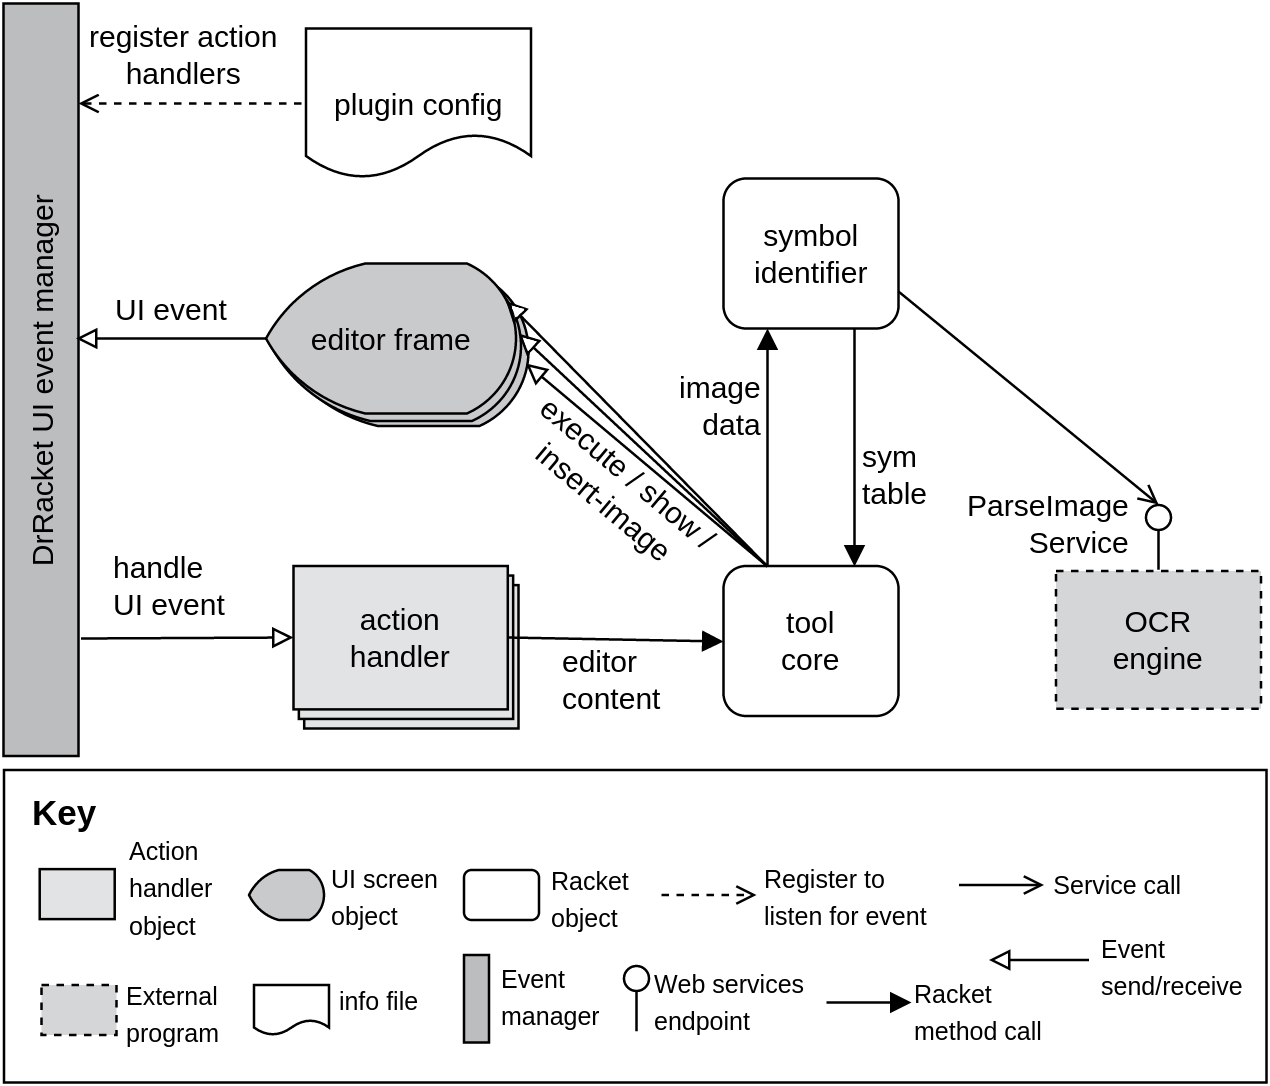
\includegraphics[scale=0.19]{img/solution}
	\vspace{-5pt}
	\caption{Diagram for a publish subscribe view of the proposed architecture.}
	\label{fig:solution}
 \vspace{-10pt}
\end{figure}

The \texttt{tool core} component, in Figure~\ref{fig:solution}, will receive, at least, three kinds of DrRacket events. For each of these events, we will change the programming environment based on the following desired action:

\begin{itemize}
	\item \texttt{on-change:} when DrRacket detects that the editor has been modified, it sends the contents of the editor over to action handlers.	The action handler, in this case, it the \texttt{online expansion handler} where the code is expanded. \textit{Desired action}: sends an \texttt{execute} event to the editor frame, if the action handler expanded the code successfully. 

	\item \texttt{on-paint:} this event is sent just before and just after every element is displayed in the editor. Handling this event provides a way to add arbitrary graphics to the editor display. \textit{Desired action}: sends a \texttt{show} event to the editor frame, to display a slider widget when the user moves the mouse over a literal.

	\item \texttt{on-new-image-snip:} this event is sent when an image is inserted in the editor. The default implementation creates an image snip which is an object with the image information, such as path and format. \textit{Desired action}: sends an \texttt{insert-image} event to the editor frame, before to get the image and send it to the \ac{ocr} engine to recognize its symbols and respective coordinates (x, y). Then, it returns a subclass of image snip, containing this extra information.
\end{itemize}

Finally, to correlate the image-snip, created above, with the function parameters we will use a syntactic transformer, i.e. macro. The macro will add a new syntax form into the language grammar, allowing an image to be used as a comment. Very similar to Lisper's comment, the macro will add a new rule in the grammar, where an image is between a function declaration and a function body (see the macro \texttt{define/img} in figure~\ref{fig:img-code}). The image will be ignored, but in background, our macro expansion will add into the function body new occurrences of the function parameters. As a result, the DrRacket syntax checker will mark these free variables and will be able to recognize bound occurrences and point to them inside an image.